\section{Exemplo Prático - Dependency Injection}
\label{sec:exemplo_di}

\begin{figure}[H]
    \centering
    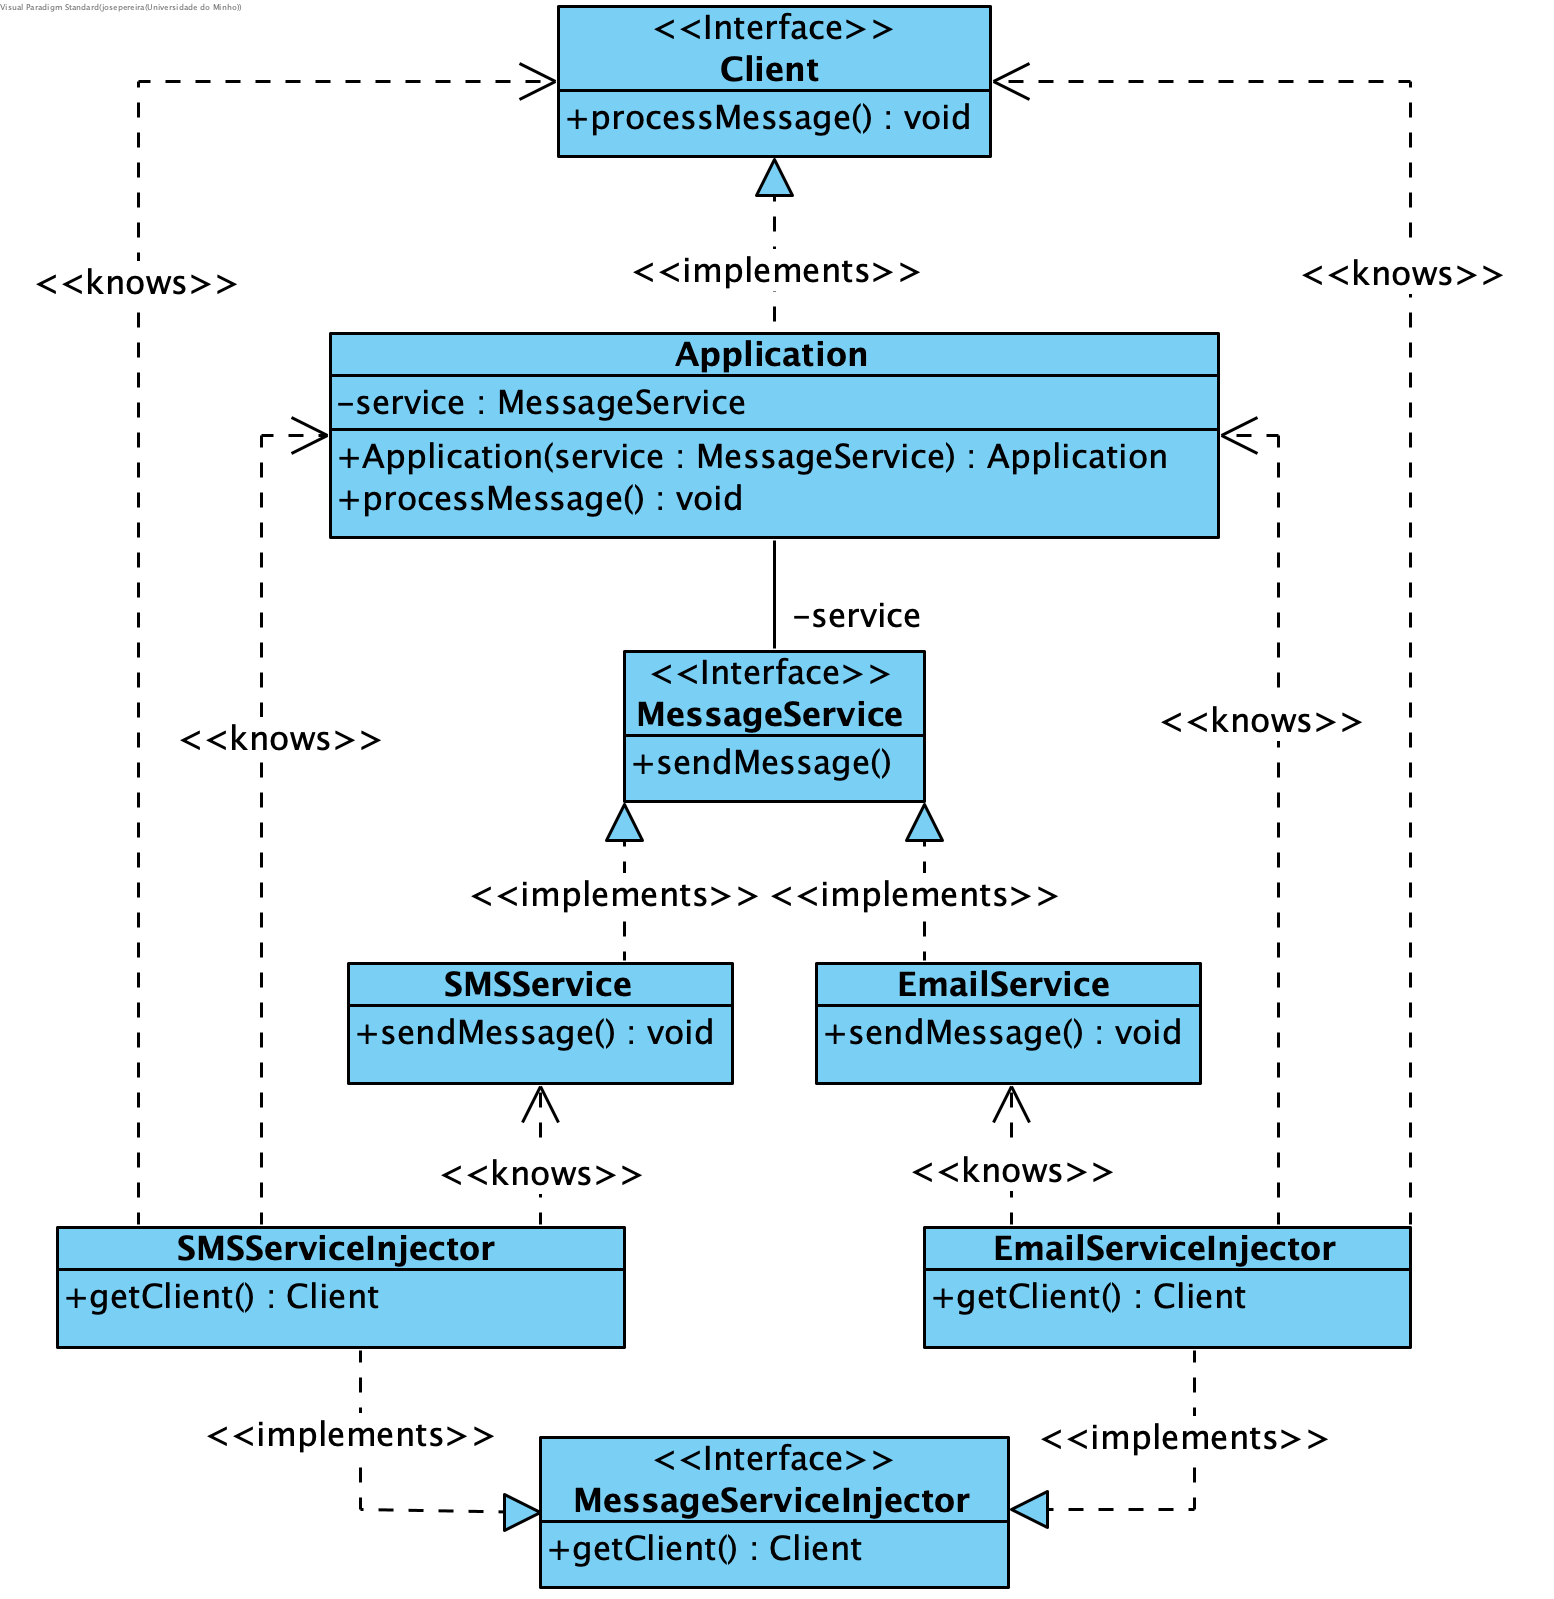
\includegraphics[scale=0.65]{images/diagram_class_dependency.png}
    \caption{Diagrama de classes da implementação.}
    \label{fig:di-exemplo}
\end{figure}

\hspace{3mm} Com a finalidade de uma melhor percepção do \textit{dependency injection}, a equipa implementou uma aplicação do mesmo a um problema real (\ref{anexo:dependency}). Desta forma, o problema em questão consiste no envio de mensagens a partir de serviços diferentes, isto é, SMS e email. Como já foi referido acima, na secção \ref{sec:dependency}, existem três entidades importantes a realçar: cliente, injector e os serviços. 

O cliente consiste na classe \textbf{Application}, que implementa a interface \textbf{Client}, este contém o serviço para o poder utilizar, no entanto, esta classe não é responsável por criar-lo, apenas conhece o seu tipo genérico, isto é, a interface \textbf{MessageService}. Ainda em relação à classe do cliente, importa realçar a importância de se ter definido o construtor, que recebe como argumento um serviço do tipo mais genérico \textbf{MessageService}, visto que, este exemplo segue o \textbf{método do construtor}, isto é, os serviços são enviados através deste, tal como foi explicado na secção \ref{sec:dependency}. 

O injector tem o papel de criar o cliente e enviar os serviços a este. Desta forma, decidiu-se definir, uma classe injectora para cada serviço, isto é, \textbf{SMSServiceInjector} e \textbf{EmailServiceInjector}. Nestas classes, existe o método \textbf{getClient()}, que tal como o nome sugere, vai criar o objecto \textbf{Client}, passando-lhe o serviço. O serviço enviado, pode ser criado no momento, ou já existir.

Os serviços, contém as funcionalidades a executar pelo cliente, sendo o seu tipo mais genérico, e que o \textbf{Client} conhece, \textbf{MessageService}. Apesar de apenas ter-se definido uma interface, segundo o diagrama da figura \ref{fig:dependency-injection}, cada serviço poderá ter uma interface independente. No entanto, para este exemplo decidiu-se definir um tipo comum para o serviço, visto que facilita o processo. A interface \textbf{MessageService}, define os métodos que se pretende que o \textbf{Client} possa utilizar do serviço, sendo neste caso o \textbf{sendMessage()}.
Cada serviço contém uma classe específica, que implementa a \textbf{MessageService} e os respectivos métodos.

Assim, o mais importante a reter deste exemplo, são os objectivos do \textit{dependency injection}, ou seja, o \textbf{Client} (\textbf{Application}), apenas usa os serviços, não os cria, e não depende da classe que os cria, isto é, as classes \textbf{injectoras} (\textbf{SMSServiceInjector} e \textbf{EmailServiceInjector}). Do mesmo modo, tal como já foi dito anteriormente, os serviços não necessitam de ser criados no momento, podem já existir. 

